\section{Experiments}
\label{sec:5}
All our experiments are reproducible with the code of our final implemented expert advisor publicly available~\footnote{https://git.l3s.uni-hannover.de/mfisichella/forex}.

\subsection{Investment Setup}
\noindent In our experiments we used the following configuration:

\begin{itemize}
\setlength\itemsep{0.3em}
\item Our investment was limited to \$ 10,000.
\item For each transaction, we allocated the amount indicated by the money management risk presented in Section~\ref{sec:tradsys} with an upper limit to 4\% of the current available capital.
\item The leverage was set to 1:30. 
\item The ideal execution for order placement with zero latency during trading execution was chosen.
\item We used a demo account with a trading broker \footnote{https://www.icmarkets.com/en/open-trading-account/demo/} simulating the placement of buy/sell positions.
\end{itemize}

\subsubsection{Evaluation Metrics}
\label{sec:metrics}
\noindent The following evaluation metrics were computed for our experiments:

\begin{itemize}
\setlength\itemsep{0.3em}
%\item \textbf{Balance:} the final financial value of the balance in terms of money.
\item \textbf{Net Profit:} the financial result (profit/loss) of all trades in terms of money.
\item \textbf{Total Trades:} the total number of trades where 1 trade includes 2 deals either by closing a long (first buy then sell) or short (first sell then buy) position.
\item \textbf{Profit Factor:} the ratio of the gross profit to the gross loss. A value of one means that these parameters are equal. The gross profit is the sum of all profitable trades in terms of money, while the gross loss is the sum of all losing trades in terms of money.
\item \textbf{Expected Payoff:} a statistically calculated value showing the average return of one deal. 
\item \textbf{Drawdown in \%:} difference between the initial deposit and the minimal level below initial deposit throughout the whole testing period.
\item \textbf{Recovery Factor:} the value reflects the riskiness of the strategy, i.e. the amount of money risked by the Expert Advisor to make the profit it obtained.
\item \textbf{Sharpe Ratio:} this ratio characterizes efficiency and stability of a strategy. It reflects the ratio of the arithmetical mean profit for the position holding time to the standard deviation from it.
\end{itemize}

\subsubsection{Datasets}
Data were collected and represent the historical data, measured at 4-hours intervals candlesticks, of 6 currency pairs: 4 major pairs like GBP/USD, EUR/USD, USD/CHF and USD/JPY, and 2 minor pairs like EUR/GBP and GBP/JPY.
Dataset spans from 01-01-2010 till 30-04-2021. Training-set was built considering data in the interval from 01-01-2010 till 31-12-2018. The remaining data constitute the test-set. Data were extracted from Metatrader 5 software, introduced in Section~\ref{sec:mt5}. 
Experiments on all 6 currency pairs are conducted on three test-sets:
\begin{itemize}
\setlength\itemsep{0.3em}
\item Entire 2019: from 01-01-2019 till 31-12-2019.
\item Entire 2020: from 01-01-2020 till 31-12-2020.
\item Current year 2021: from 01-01-2021 till 30-04-2021.
\end{itemize}

Trading rules are active on each candlesticks, but as soon as a position is open and on the market, our approach check each tick of the market. A tick is an event characterized by a new price for a symbol at some moment; ticks are more frequent than candlesticks. In Table~\ref{tab:ticks}, we report the number of ticks for each test set intervals.

 \begin{table}[h!]
    \caption{Test-set data details.}
  \begin{center} 
    \label{tab:ticks}
    \begin{tabular}{c c c c }
    \hline
    \multirow{2}{*}{\centering \textbf{Currency Pairs}} &  \textbf{2019}  &  \textbf{2020}&  \textbf{2021}\\\cline{2-4} % <-- Combining 2 rows with arbitrary with (*) and content 12
         & Ticks  & Ticks  & Ticks\\ % <-- Content of first column omitted.
      \hline
        EUR/USD   & 14,107,144   & 22,493,176  & 6,418,430\\
        USD/CHF     & 13,057,137   & 15,598,601  & 4,256,816\\
        USD/JPY    & 16,510,745  & 19,068,209   & 4,487,949\\
        EUR/GBP    &  15,810,439 & 19,224,884  & 5,481,037\\
        GBP/JPY   &  32,155,222 & 35,299,958  & 9,181,770\\
        GBP/USD    & 20,904,274  & 24,012,594  & 7,117,293\\
	\hline
    \end{tabular}
  \end{center}
\end{table}

\subsection{Results on Phase 1}
The goal of the first phase is the selection of trading rules: rules whose best chromosome does not have a positive net profit are directly eliminated and do not pass to the second phase.
In Table~\ref{tab:qualrules}, we report the qualified and unqualified trading rules.

\begin{table}[h!]
  \begin{center} 
    \caption{Unqualified and qualified trading rules.}
    \label{tab:qualrules}
    \begin{tabular}{p{6cm}  p{6cm} }
    \hline
    \multicolumn{2}{c}{\textbf{Rule Name}}
    \\\cline{1-2}
    \textbf{Unqualified Rules} & \textbf{Qualified Rules}\\
    \hline
    Adaptive Moving Average, Donchian channel, Stoller Bands,  Double Exponential Moving Average, Envelope Moving Avarage,  Fractal Adaptive Moving Avarage, Triple Exponential Moving Average, Avarage True Range,  MACD (Moving Average Convergence Divergence),  William' Percentage Range, Momentum, RSI (Relative Strength Index). 
    &
    Average Directional Moving Index, Bollinger Bands, Standard Deviation, Parabolic SAR, Bears Power, Bulls Power, Stochastic oscillator, Heiken Ashi Candles.\\
      \hline
    \end{tabular}
  \end{center}
\end{table}

\subsection{Results on Phase 2: without AI-based}
In the second phase, profitable rules among the qualified rules are selected and combined. The final output is the best chromosomes having the highest Net Profit.
The best chromosome output the combination of the following rules: Bollinger Bands, Stochastic oscillator, Bears Power, Bulls Power, and Heiken Ashi Candles. According to this combination, we implemented the expert advisor for trading. 

The results of the experiments using all metrics presented in Section~\ref{sec:metrics} are reported in Table~\ref{tab:expyears}. For almost all currency pairs during the three long considered time intervals we are profitable and the results show that the best strategy is to invest simultaneously on all of the currency to reduce the loss risk and stay profitable. %The outcomes highlighted how our approach can achieve profit yearly based from +35\% to +155\%.

\begin{table}[h!]
    \caption{Experiments on several datasets. In green the net profit, in red the net loss. }
  \begin{adjustwidth}{-.7in}{-.5in}  
  \begin{center} 

    \label{tab:expyears}
    \begin{tabular}{p{2.4cm} c c p{2.5em} p{2.9em} p{3.4em}  p{3.7em} p{3em} p{3.1em}  p{2.5em} }
    \hline
    \multirow{2}{*}{\centering \textbf{Date}} & \multirow{2}{*}{\textbf{Currency Pairs}} &  \multicolumn{7}{c}{\textbf{Metrics}}\\\cline{3-9} % <-- Combining 2 rows with arbitrary with (*) and content 12
   
      &   & Net Profit & Total Trades & Profit Factor & Expected Payoff & Drawdown in \% & Recovery Factor & Sharpe Ratio\\ % <-- Content of first column omitted.
      \hline
       \multirow{6}{*}{\parbox{3cm}{\centering \textbf{2019 \\ (01.01. - 31.12.)}}} & GBP/USD  & {\color{OliveGreen} 1490.90} & \centering 74 & 1.19 & 20.15 & 19.18 & 0.57 & 0.09\\
       & EUR/USD  & {\color{OliveGreen} 3470.01} & \centering 46 & 1.87 & 75.43 & 12.83 & 1.78 & 0.28\\
       & USD/CHF  & {\color{OliveGreen} 2466.51} & \centering 47 & 1.54 & 52.48 & 9.91 & 2.33 & 0.18\\
       & USD/JPY  & {\color{BrickRed} -175.52} & \centering 51 & 0.96 & -3.44 & 15.56 & -0.11 & -0.01\\
       & EUR/GBP  & {\color{BrickRed} -986.34} & \centering 62 & 0.85 & -15.91 & 20.53 & -0.44 & -0.05\\
       & GBP/JPY  & {\color{OliveGreen} 117.27} & \centering 89 & 1.01 & 1.32 & 19.34 & 0.05 & 0.02\\
       \hline
	\textbf{Yearly Total} &  & {\color{OliveGreen} \textbf{6382.83}} & & & & & \\
	\hline
	\hline
       \multirow{6}{*}{\parbox{3cm}{\centering \textbf{2020 \\ (01.01. - 31.12.)}}} & GBP/USD &  {\color{OliveGreen} 3883.91} & \centering 102 & 1.44 & 38.08 & 11.66 & 2.79 & 0.16\\
       & EUR/USD  & {\color{OliveGreen} 884.04} & \centering 78 & 1.12 & 11.33 & 18.13 & 0.40 & 0.06\\
       & USD/CHF & {\color{OliveGreen} 1172.22} & \centering 68 & 1.18 & 17.24 & 12.82 & 0.73 & 0.08\\
       & USD/JPY  & {\color{OliveGreen} 1552.46} & \centering 66 & 1.29 & 23.52 & 11.70 & 1.24 & 0.11\\
       & EUR/GBP & {\color{OliveGreen} 4526.89} & \centering 71 & 1.77 & 63.76 & 12.45 & 2.95 & 0.23\\
       & GBP/JPY  & {\color{OliveGreen} 3438.72} & \centering 97 & 1.50 & 35.45 & 11.22 & 2.53 & 0.17\\
    \hline
	\textbf{Yearly Total} &   & {\color{OliveGreen} \textbf{15458.24}} & & & & & \\
	\hline
	\hline
      
       \multirow{6}{*}{\parbox{3cm}{\centering \textbf{2021 \\ (01.01. - 30.04.)}}} & GBP/USD &  {\color{BrickRed} -48.82} & \centering 27 & 0.98 & -1.81 & 11.11 & -0.04 & 0.00\\
       & EUR/USD & {\color{BrickRed} -714.86} & \centering 21 & 0.67 & -34.04 & 11.60 & -0.61 & -0.15\\
       & USD/CHF  & {\color{BrickRed} -260.77} & \centering 20 & 0.87 & -13.04 & 9.61 & -0.27 & -0.05\\
       & USD/JPY  & {\color{OliveGreen} 2301.49} & \centering 13 & 3.58 & 177.04 & 7.02 & 2.63 & 0.55\\
       & EUR/GBP  & {\color{OliveGreen} 1368.48} & \centering 14 & 2.06 & 97.75 & 8.81 & 1.42 & 0.30\\
       & GBP/JPY  & {\color{OliveGreen} 900.31} & \centering 29 & 1.30 & 31.05 & 20.99 & 0.38 & 0.12\\
     \hline
	\textbf{Yearly Total} &   & {\color{OliveGreen} \textbf{3545.83}} & & & & & \\
	\hline
	\hline
    \end{tabular}
  \end{center}
  \end{adjustwidth}
\end{table}

For sake of clarity, we also present the temporal investment graph for all 6 currency pairs conducted on the three test-sets: Fig.~\ref{fig:2019} for 2019, Fig.~\ref{fig:2020} for 2020, and Fig.~\ref{fig:2021} for 2021. In details, we report the Balance/Equity chart and the Deposit load chart.

Balance shows the amount of deposited money in our trading account. The profit/loss of our orders will be added or deducted to/from our trading account balance when we close our orders.
Balance and Equity show the same values as long as there is not any open order. When we have open orders in our trading account, the Balance will not change and it will stay fixed but the Equity will be floated according to the profit/loss of our current orders. 

The deposit load value shows the percent of account funds used to open positions. 
If the current account value is \$ 10,000 and the margin of open positions is \$ 5,000, the account load is 50\% = \$5,000 / \$ 10,000 * 100\%. Larger traded lot values cause larger equity fluctuations on the provider's account in case of market price changes, resulting in a larger load on the trading account. In other words, the higher the load on the account, the higher the risks.
Margin depends on the account leverage, which means that the load on an account with the 1:500 leverage will be 5 times less than that on the account with the 1:100 leverage. But the risk will be the same. In our experiment the deposit load was always below 25\%.

\begin{figure}[h]
  \centering
  \subfloat[][GBP/USD]{\label{fig:flickr}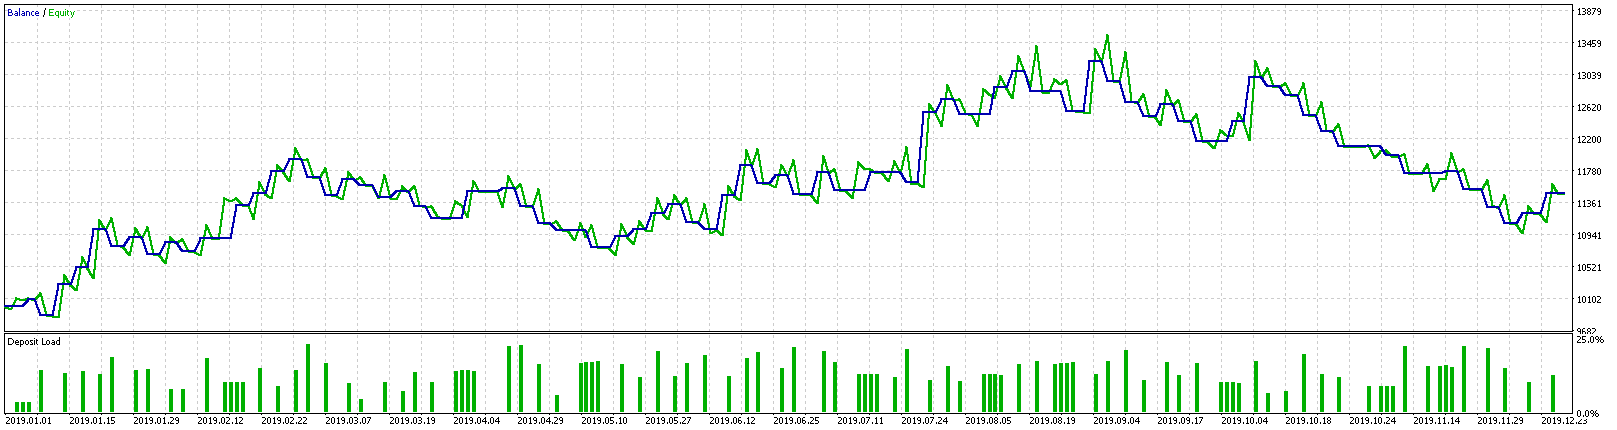
\includegraphics[width=.77\textwidth]{2019_GBPUSD.png}} \\[-.1ex]   
  \subfloat[][EUR/USD]{\label{fig:flickr}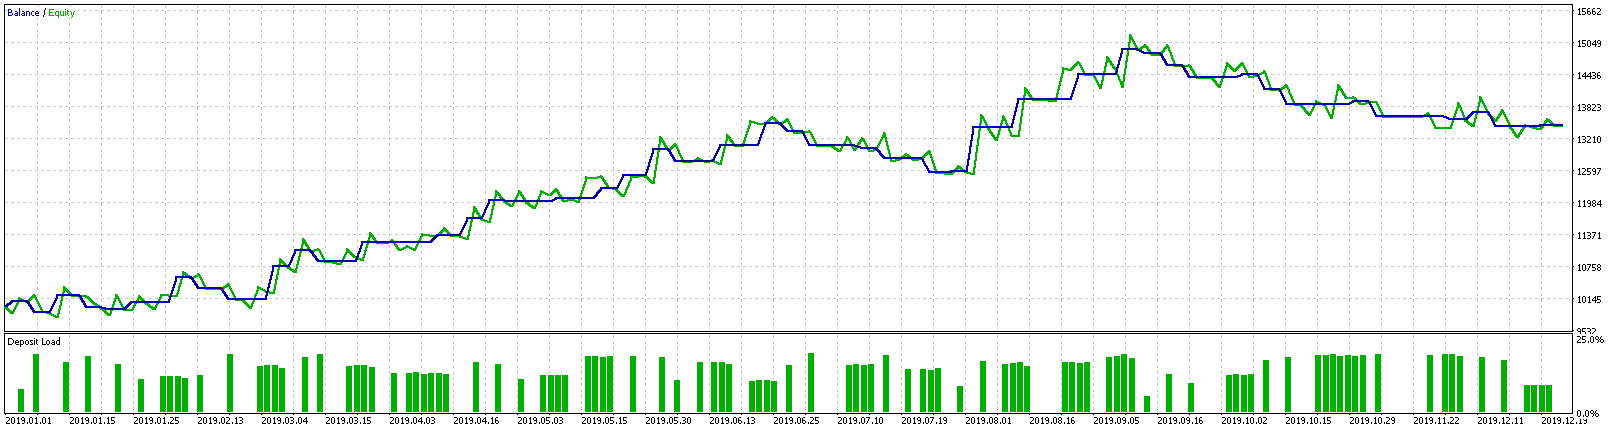
\includegraphics[width=.77\textwidth]{2019_EURUSD.png}}  \\[-.1ex]  
  \subfloat[][USD/CHF]{\label{fig:flickr}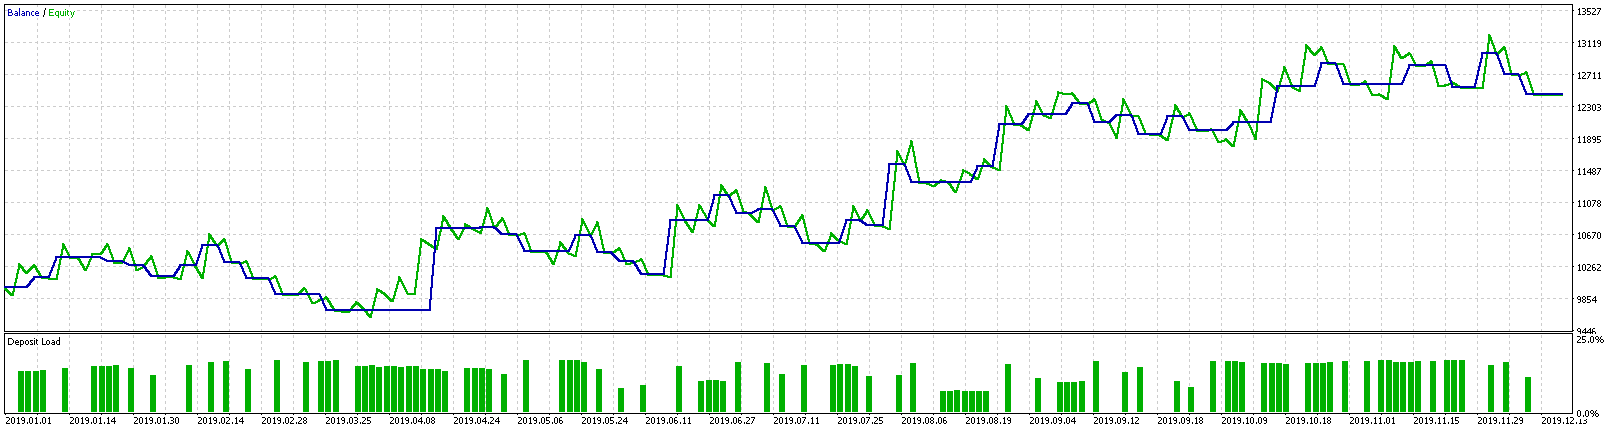
\includegraphics[width=.77\textwidth]{2019_USDCHF.png}} \\   [-.1ex]  
  \subfloat[][USD/JPY]{\label{fig:flickr}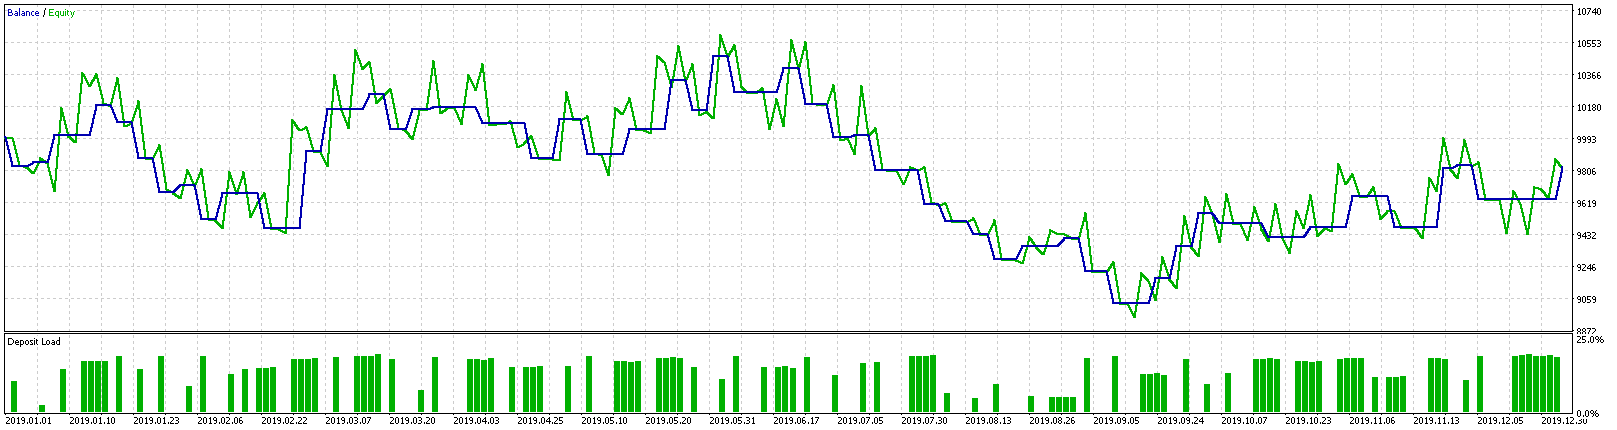
\includegraphics[width=.77\textwidth]{2019_USDJPY.png}} \\   [-.1ex]  
  \subfloat[][EUR/GBP]{\label{fig:flickr}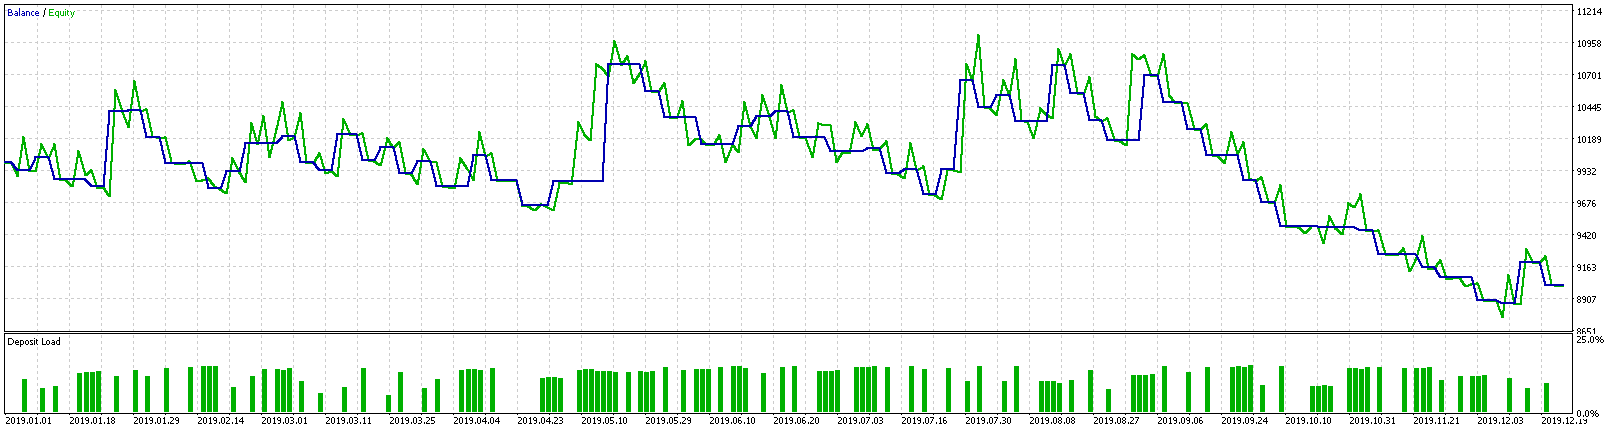
\includegraphics[width=.77\textwidth]{2019_EURGBP.png}} \\  [-.1ex]              
  \subfloat[][GBP/JPY]{\label{fig:tiny}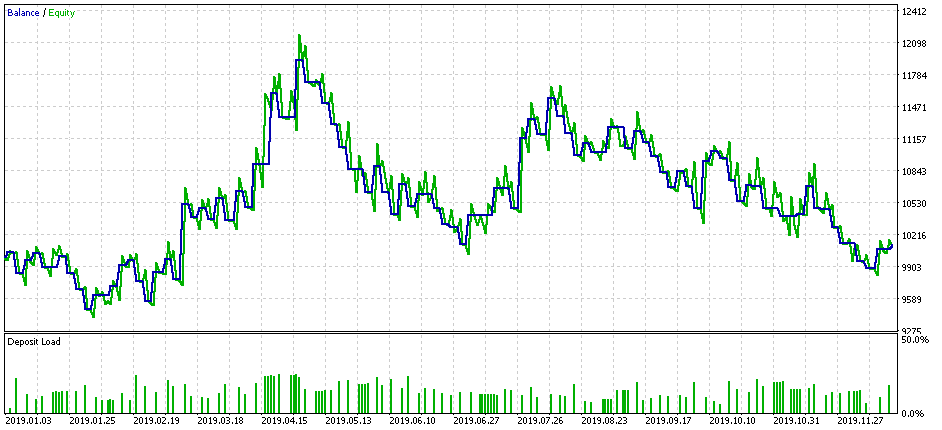
\includegraphics[width=.77\textwidth]{2019_GBPJPY.png}}  \\  [-.1ex]    
  \caption{Balance/Equity Graphs and Deposit Load for the entire 2019}
  \label{fig:2019}
\end{figure}

\begin{figure}[h]
  \centering
  \subfloat[][GBP/USD]{\label{fig:flickr}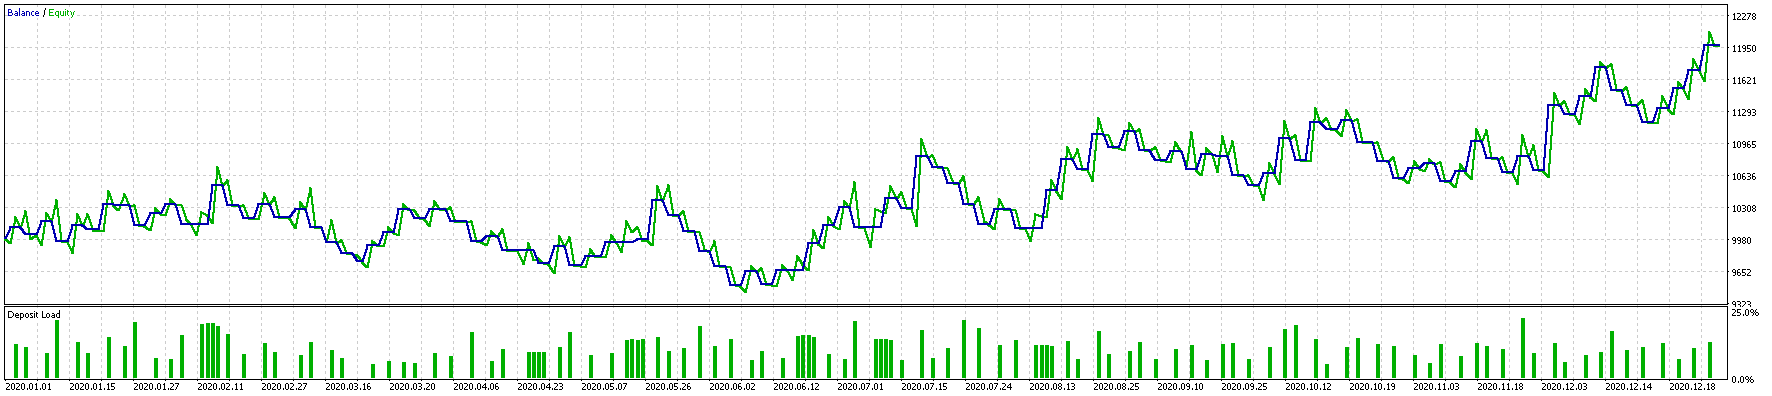
\includegraphics[width=.77\textwidth]{2020_GBPUSD.png}} \\[-.1ex]   
  \subfloat[][EUR/USD]{\label{fig:flickr}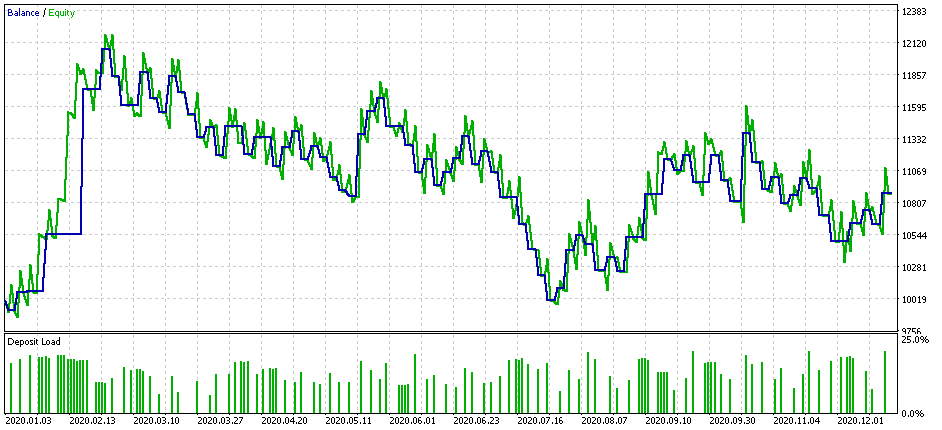
\includegraphics[width=.77\textwidth]{2020_EURUSD.png}}  \\[-.1ex]  
  \subfloat[][USD/CHF]{\label{fig:flickr}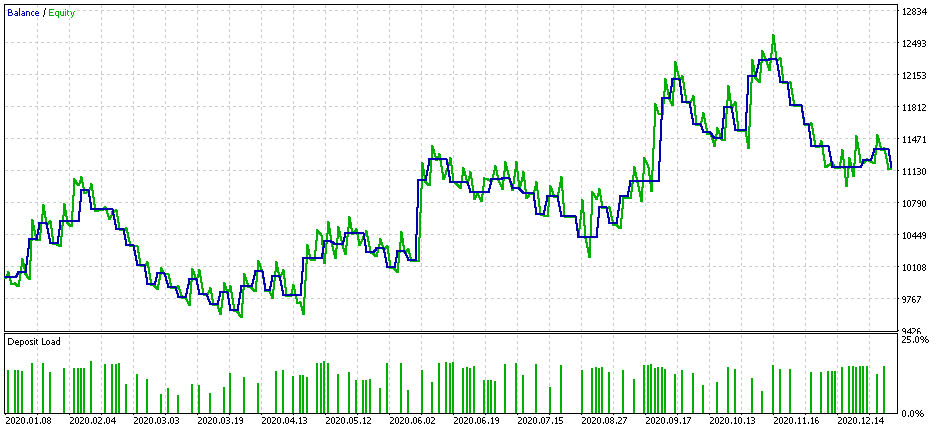
\includegraphics[width=.77\textwidth]{2020_USDCHF.png}} \\   [-.1ex]  
  \subfloat[][USD/JPY]{\label{fig:flickr}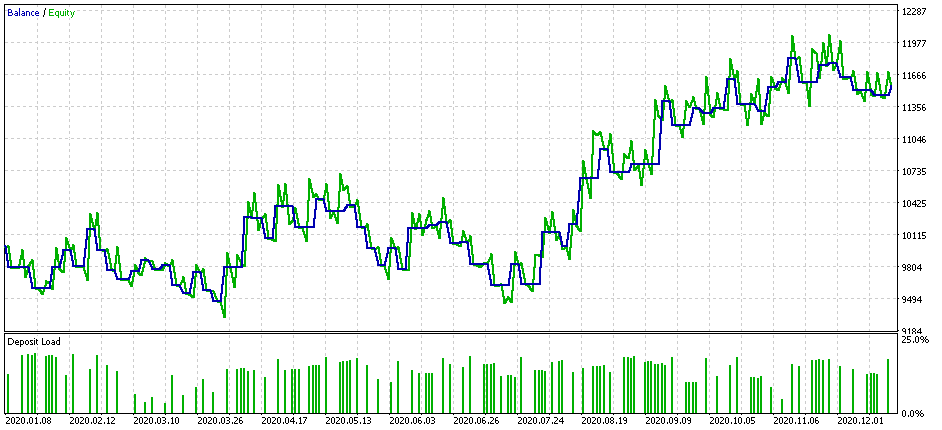
\includegraphics[width=.77\textwidth]{2020_USDJPY.png}} \\   [-.1ex]  
  \subfloat[][EUR/GBP]{\label{fig:flickr}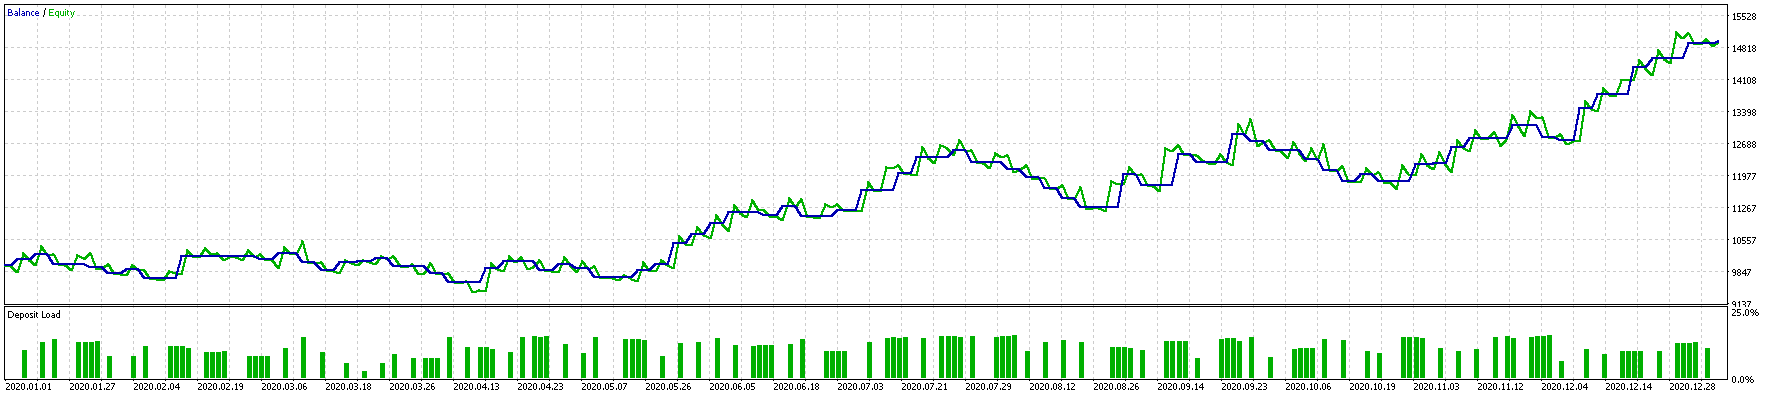
\includegraphics[width=.77\textwidth]{2020_EURGBP.png}} \\  [-.1ex]              
  \subfloat[][GBP/JPY]{\label{fig:tiny}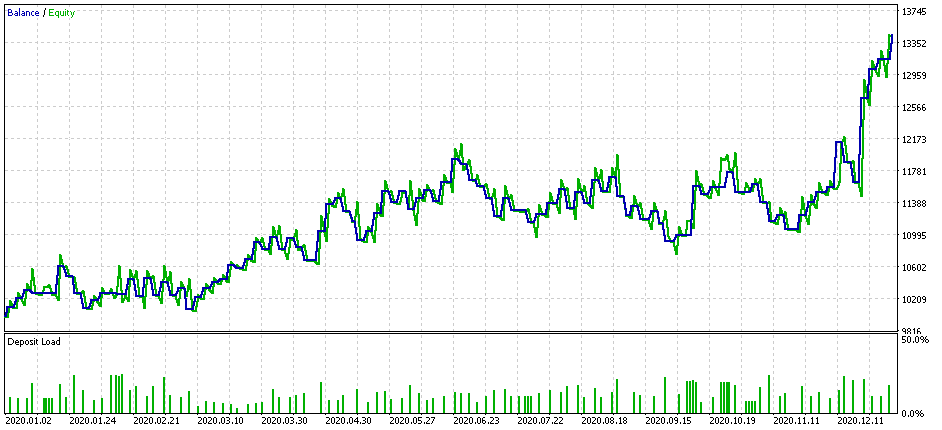
\includegraphics[width=.77\textwidth]{2020_GBPJPY.png}}  \\  [-.1ex]    
  \caption{Balance/Equity Graphs and Deposit Load for the entire 2020}
  \label{fig:2020}
\end{figure}

\begin{figure}[h]
  \centering
  \subfloat[][GBP/USD]{\label{fig:flickr}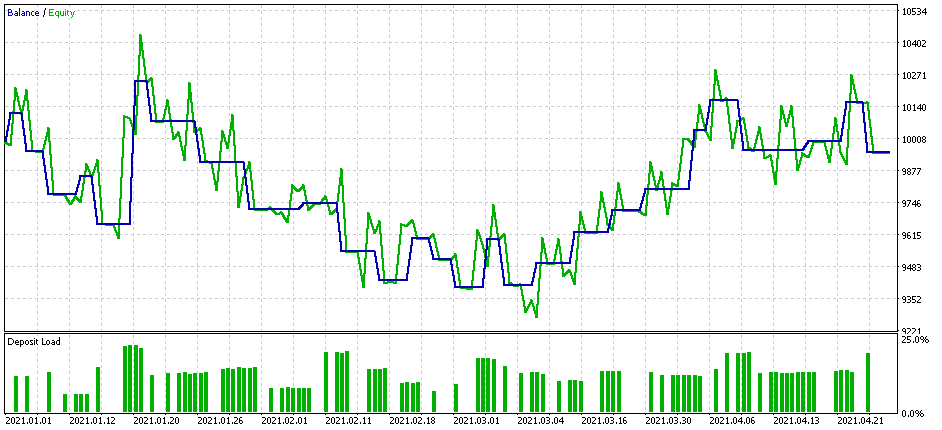
\includegraphics[width=.77\textwidth]{2021_GBPUSD.png}} \\[-.1ex]   
  \subfloat[][EUR/USD]{\label{fig:flickr}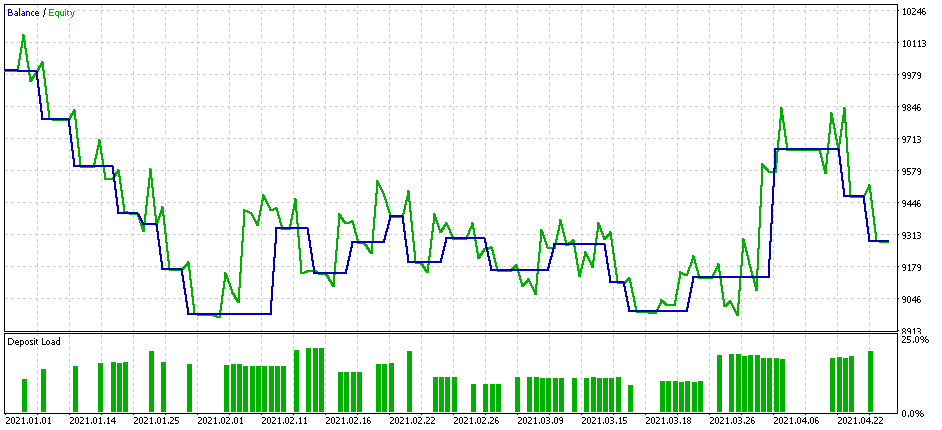
\includegraphics[width=.77\textwidth]{2021_EURUSD.png}}  \\[-.1ex]  
  \subfloat[][USD/CHF]{\label{fig:flickr}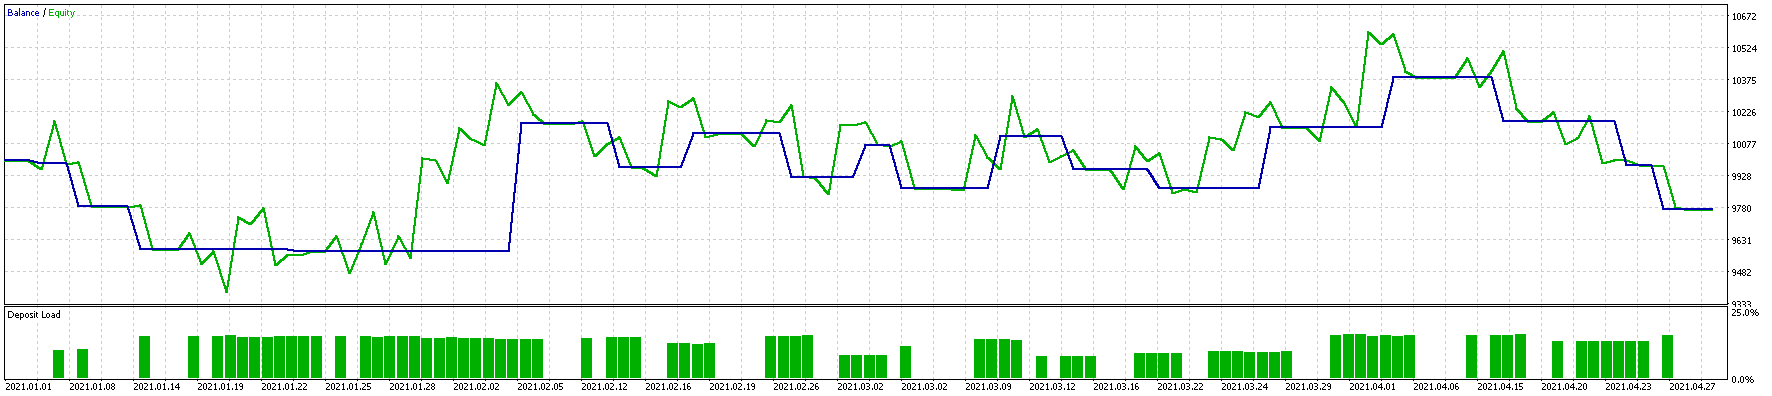
\includegraphics[width=.77\textwidth]{2021_USDCHF.png}} \\   [-.1ex]  
  \subfloat[][USD/JPY]{\label{fig:flickr}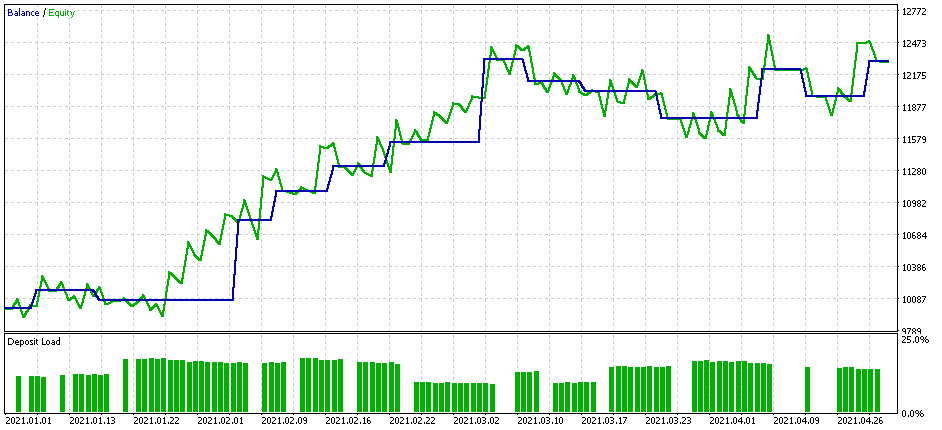
\includegraphics[width=.77\textwidth]{2021_USDJPY.png}} \\   [-.1ex]  
  \subfloat[][EUR/GBP]{\label{fig:flickr}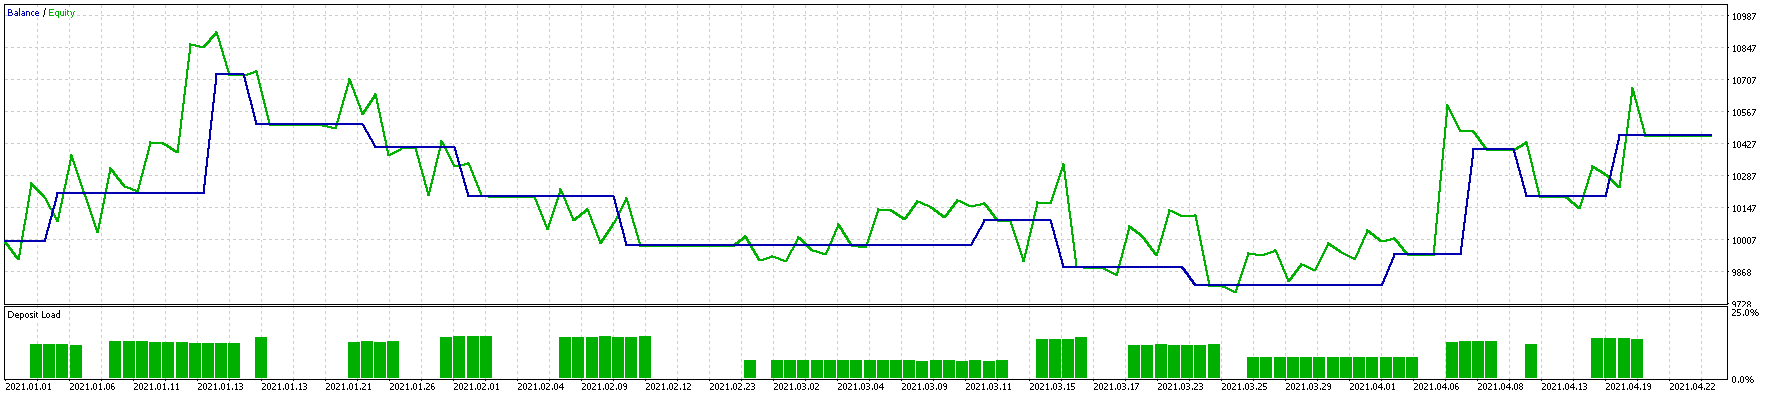
\includegraphics[width=.77\textwidth]{2021_EURGBP.png}} \\  [-.1ex]              
  \subfloat[][GBP/JPY]{\label{fig:tiny}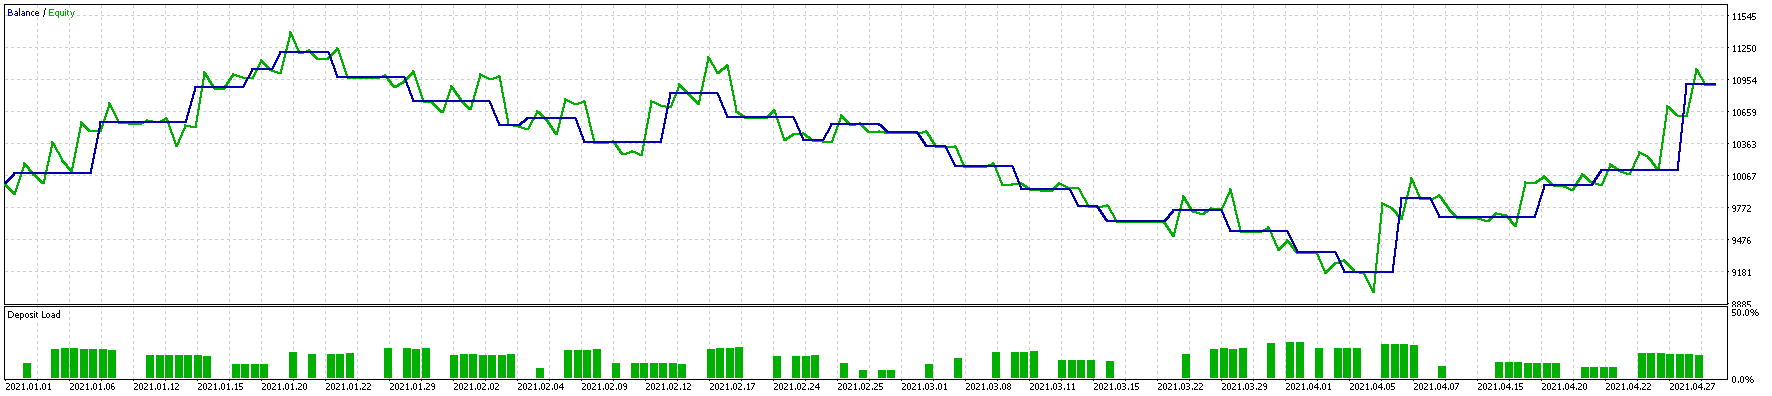
\includegraphics[width=.77\textwidth]{2021_GBPJPY.png}}  \\  [-.1ex]    
  \caption{Balance/Equity Graphs and Deposit Load for 2021, from 01.01 until 30.04}
  \label{fig:2021}
\end{figure}

\subsection{Results on Phase 2: including AI-based}


\subsection{AI Convolutional Layer}

\subsubsection{Experimental Setup}

\subsubsection{Evaluation Metrics}

\subsubsection{Dataset}

\subsubsection{Results} 

